\documentclass[11p]{article}
% Packages
\usepackage{amsmath}
\usepackage{graphicx}
\usepackage[swedish]{babel}
\usepackage[
    backend=biber,
    style=authoryear-ibid,
    sorting=ynt
]{biblatex}
\usepackage[utf8]{inputenc}
\usepackage[T1]{fontenc}
%Källor
\addbibresource{mall.bib}
\graphicspath{ {./images/} }

\title{PMmall \\ \small Fysik 1}
\author{Gabriel Nilsson Högberg}
\date{\today}

\begin{document}

    \begin{titlepage}
        \begin{center}
            \vspace*{1cm}

            \Huge
            \textbf{Avfall som energiförsörjning}

            \vspace{0.5cm}
            \LARGE
            Biobränsle

            \vspace{1.5cm}

            \textbf{Gabriel Nilsson Högberg}

            \vfill

            Ett PM om energiförsörjning \\
            Fysik 1

            \vspace{0.8cm}

            
\includegraphics[width=0.4\textwidth]{../images/NTI Gymnasiet_Symbol_print_svart.png}

            \Large
            Teknikprogrammet\\
            NTI Gymnasiet\\
            Umeå\\
            \today

        \end{center}
    \end{titlepage}
    \tableofcontents
    \newpage

    \section{Inledning}
    Ämnet handlar om avfall som energiförsörjning, alltså sopor som bränns för att bilda värme och el. Det som är viktigt att veta är hur detta funkar och hur detta påverkar miljön och samhället både lokalt och globalt.

    \subsection{frågeställningar}
    De frågorna som ska besvaras är följande:
    \begin{enumerate}
        \item Hur fungerar avfallsförbränning?
        \item Vilken sorts miljöpåverkan har avfallsförbränning lokalt och globalt?
        \item Hur påverkar avfallsförbränning samhället lokalt och globalt?
    \end{enumerate}

    \section{Resultat}
    \subsection{Avfallsförbränning, så fungerar det}
    \begin{figure}[!h]
        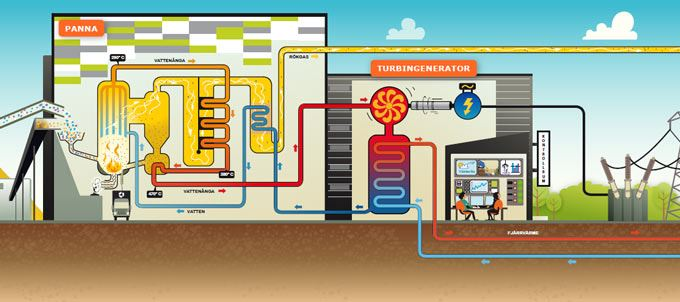
\includegraphics[width=0.8\textwidth]{../images/avfallförbränning.jpg}
        \caption{En bild av hur förbränning av avfall fungerar. Källa: Malarenergi.se}
        \label{fig:avfallsforbranning}
    \end{figure}
    Enligt \textcite{SoporNu} fungerar avfallsförbränning genom att man har avfallseldade kraftvärmeverk som ska kunna producera både värme och el genom att bränna sopor.
    I själva kraftvärmeverket överförs värme av rökgaser till vatten som bildar ånga och som i sin tur driver en turbin för elproduktion.
    Sedan förs den resterande energin till fjärrvärmenätet som värmer hushåll i Sverige.
    Detta visas även i figuren~\ref{fig:avfallsforbranning}
    \subsection{Lokala och globala miljöpåverkningar av avfallsförbränning}
    Vid förbränningsprocessen av avfall frigörs framförallt koldioxid och vatten och enligt \textcite{AvfallSverige} är det ett hygieniskt och miljömässigt bra sätt eftersom vi har otroligt bra reningstekniker och förbränningsförhållanden samtidigt som vi har bra kontroll av att inte släppa ut föroreningar av avfallsförbränningen.
    Idag kan man också nästan helt få rökgaserna som släpps ut att bestå av 99,9 procent ämnen som redan finns i luften, det vill säga kväve, vattenånga, koldioxid och syre.

    \newline

    Det finns däremot stora negativa påverkningar av miljön. Enligt \textcite{naturvardsverket} är bränderna svårsläckta och kan pågå i flera veckor och dem kan fortfarande släppa ut farliga gaser även fast vi har bra reningstekniker. Dessutom där soporna hamnar kallas för en deponi (soptip) och dessa samlar stora mängder föroreningar och miljögifter som sedan förs vidare av lakvatten, vatten från regn som därefter för dessa dåliga ämnen vidare. Själva deponierna ger upphov till utsläpp av ämnet metangas som i sig är en av dem värsta växthusgaserna. Metangas har nästan 25 gånger större påverkan än koldioxid och detta är ett av Europas största miljöproblem enligt \textcite{Vattenfall}.
    \subsection{Hur avfallsförbränning påverka samhället lokalt och globalt}
    Påverkan i samhällen både lokalt och globalt är väldigt positivt eftersom enligt \textcite{stockholmenergi} fungerar avfallsförbränning i samhällen som njurar.
    Det innebär som riktiga njurar att dessa anläggningar sorterar bort farliga ämnen ur kretsloppet.
    I med att det fungerar som njurar är det då viktigare i långsikt också att ta bort dessa ämnen i samhällen.

    \section{Slutsatser}
    Här kan du dra slutsatser eller sammanfatta ditt resultat

    Citat skrivs mellan de konstiga symbolerna \verb|``| och \verb|''| för att de ska se bra ut ``se bra ut!''.


    \printbibliography

\end{document}
